%%%%%%%%%%%%%%%%%%%%%%%%%%%%%%%%%%%%%%%%%%%%%%%%%%%%%%%%%%%%%%
%% Carlos Segarra's Beamer Presentation Template. All credits
%% to Vincent Labatut from whom I took the template and added
%% my own flavour to it. Kudos to <vincent.labatut@univ-avignon.fr>
%%%%%%%%%%%%%%%%%%%%%%%%%%%%%%%%%%%%%%%%%%%%%%%%%%%%%%%%%%%%%%
% setup Beamer
\documentclass[10pt,    % default is 11pt, use 10pt for more compact slides
%    handout,            % collapse all overlays (=animations) and video-invert console text
    english,            % presentation language (theme supports only french & english)
    xcolor=table,       % colors in the tables
    envcountsect,        % include section number in theorem numbers
    aspectratio=169     % Using 16:9 aspect ratio because 2019
]{beamer}

%%%%%%%%%%%%%%%%%%%%%%%%%%%%%%%%%%%%%%%%%%%%%%%%%%%%%%%%%%%%%%
% setup the theme
%\usepackage{au/sty/beamerthemeAU}         % no option at all
\usepackage[light]{csg-temp/sty/beamerthemeAU}   % the "light" option only changes the title and section pages

%%%%%%%%%%%%%%%%%%%%%%%%%%%%%%%%%%%%%%%%%%%%%%%%%%%%%%%%%%%%%%
% setup side notes
\usepackage{pgfpages}                                   % comment all 3 below lines to hide notes
%\setbeameroption{show notes}                           % alternate content and note slides
%\setbeameroption{show only notes}                      % only note slides
%\setbeameroption{show notes on second screen=right}    % dualscreen: right, left, top, bottom
%\usepackage{enumitem}

%%%%%%%%%%%%%%%%%%%%%%%%%%%%%%%%%%%%%%%%%%%%%%%%%%%%%%%%%%%%%%
% name of the biblatex file
\addbibresource{biblio.bib}

%%%%%%%%%%%%%%%%%%%%%%%%%%%%%%%%%%%%%%%%%%%%%%%%%%%%%%%%%%%%%%
% External Packages
\usepackage{datenumber}
\usepackage{varwidth}
%\usepackage[ruled]{algorithm2e}

% Math Mode
%\usepackage{algorithm}
%\usepackage{algorithmic}
%\usepackage{algorithm2e}
%\usepackage{multicol}
%\usepackage[noend]{algpseudocode}

%%%%%%%%%%%%%%%%%%%%%%%%%%%%%%%%%%%%%%%%%%%%%%%%%%%%%%%%%%%%%%
% title and subtitle of the presentation (the latter is optional)
\subtitle{Decentralized Systems} % leave empty if no subtitle
\title[Decentralized Systems] % leave empty for no title in footer
    {\normalsize Gossip Protocols \\ \Large \textsc{T-Man:} Gossip-based \\ \Large Overlay Topology Management}
\subtitle{Master in Research in Informatics - MIRI}
%%%%%%%%%%%%%%%%%%%%%%%%%%%%%%%%%%%%%%%%%%%%%%%%%%%%%%%%%%%%%%
% date of the presentation (leave empty for no date, default is today)
\date[April 24th, 2020] % leave empty for no date in footer
    {Friday April 24th, 2020}
    %{\datedayname, \today}
%%%%%%%%%%%%%%%%%%%%%%%%%%%%%%%%%%%%%%%%%%%%%%%%%%%%%%%%%%%%%%
% authors and their affiliations (the latter is optional)
\author[] % leave empty for no author in footer
{M. Jelasity, and O. Babaoglu \\\small \textit{Presented by} Carlos Segarra - \texttt{carlos.segarra@estudiant.upc.edu}}
%{\inst{1} Computer Science Lab, Avignon University -- LIA EA 4128 \texttt{\{firstname.lastname\}@univ-avignon.fr}
%\and \inst{2} Institute of Disruptive Innovation, University of Excellence \texttt{\{firstname.lastname\}@univ-excell.fr}
%}
%%%%%%%%%%%%%%%%%%%%%%%%%%%%%%%%%%%%%%%%%%%%%%%%%%%%%%%%%%%%%%
% optional: additional logo (ex. lab)
%\titlegraphic{
\includegraphics[width=3cm,]{images/logo_FME.png}}
% if you want several logos, put them in a box
%\titlegraphic{\parbox{3cm}{\includegraphics[width=3cm,]{images/ceri_logo.pdf}\newline\includegraphics[width=3cm,]{images/lia_logo.pdf}}}
%%%%%%%%%%%%%%%%%%%%%%%%%%%%%%%%%%%%%%%%%%%%%%%%%%%%%%%%%%%%%%

%%%%%%%%%%%%%%%%%%%%%%%%%%%%%%%%%%%%%%%%%%%%%%%%%%%%%%%%%%%%%
% Presentation speciphic packages
% \usepackage{multicol}
% \usepackage[titles]{tocloft}
% \renewcommand{\cftchapfont}{\normalfont\bfseries}
\usetikzlibrary{decorations.pathmorphing, patterns}
\usepackage{tabularx}
\newcolumntype{L}[1]{>{\raggedright\arraybackslash}p{#1}}
\newcolumntype{C}[1]{>{\centering\arraybackslash}p{#1}}
\newcolumntype{R}[1]{>{\raggedleft\arraybackslash}p{#1}}
%%%%%%%%%%%%%%%%%%%%%%%%%%%%%%%%%%%%%%%%%%%%%%%%%%%%%%%%%%%%%

%%%%%%%%%%%%%%%%%%%%%%%%%%%%%%%%%%%%%%%%%%%%%%%%%%%%%%%%%%%%%%
\begin{document}
%%% title page
\begin{frame}
  \titlepage
\end{frame}

\begin{frame}
    \frametitle{General Information}

    \begin{itemize}
        \item \textbf{Full Title:} "\textsc{T-Man:} Gossip-based Overlay Topology Management" $[1]$
        \item \textbf{Authors:} M\'ark Jelasity and Ozalp Babaoglu
        \item \textbf{Published At:} International Workshop on Engineering Self-Organising Applications
 - ESOA 2005
        \item \textbf{DOI:} \href{https://doi.org/10.1109/WoWMoM.2011.5986177}{10.1109/WoWMoM.2011.5986177}
    \end{itemize}


    \small
    \begin{description}
        \item $[1]$ Jelasity, Márk and Babaoglu, Ozalp. (2006). T-Man: Gossip-Based Overlay Topology Management. 3910. 1-15. 
    \end{description}
 

\end{frame}

\begin{frame}
    \frametitle{TL-DR}
    \framesubtitle{A Ten Thousand Feet View}

    \vspace{-25pt}

    \begin{alertblock}{Main Contribution}
        The paper presents \textsc{T-Man} a \textbf{gossip-based protocol} to address the \textbf{topology management problem} in large-scale, dynamic networks.
    \end{alertblock}

    \begin{block}{Techniques}
        The authors introduce a generalized per-node \textbf{ranking function} to sort the set of peers even in the presence of \textbf{network churn}.
    \end{block}

    \begin{alertblock}{Evaluation Results}
        Results show a \textbf{logarithmic} dependence between the convergence rate and the network size, and a good reliability in the presence of high churn rates.
    \end{alertblock}

\end{frame}

\begin{frame}
    \frametitle{Background Concepts}
    \framesubtitle{Gossip-Based Protocols}

    \textbf{Gossip Protocol:}
    \begin{itemize}
        \item A \textbf{\textcolor{blue}{gossip protocol}} is a procedure of computer peer-to-peer communication.
        \item It is based on the way \textbf{epidemics} spread (very handy).
        \item Each node disseminates the information to communicate to all it's neighbours. Effectively \textbf{flooding} the network.
    \end{itemize}
    \textbf{Some Examples:}
    \begin{itemize}
        \item \href{https://en.wikipedia.org/wiki/Tribler}{Tribler:} is a BitTorrent peer to peer client using gossip protocols.
        \item Gossip protocols are used to achieve and maintain distributed databases' consistency.
        \item Gossip protocols are also widely used in routing.
    \end{itemize}

\end{frame}

\begin{frame}
    \frametitle{Background Concepts}
    \framesubtitle{Topology Management Problem}

    \vspace{-20pt}
    \begin{columns}
        \begin{column}{.65\textwidth}
            \textbf{The Topology Management Problem:}
            \begin{itemize}
                \item There are a set of \textcolor{blue}{\textbf{nodes}} connected through a routed network. Each node has:
                \begin{itemize}
                    \item A uniquely identifiable address \texttt{c}
                    \item A node descriptor object with relevant information.
                    \item A \textbf{partial view}: a subset of the nodes.
                \end{itemize}
                \item The set of partial views make up the \textcolor{blue}{\textbf{overlay network topology}}.
            \end{itemize}
            \textbf{Topology Management Problem:}
            \begin{itemize}
                \item How to dynamically modify the \textit{partial views} so that the overlay network converges to a \textbf{target topology}?
            \end{itemize}
        \end{column}
        \hfill
        \begin{column}{.35\textwidth}
            \begin{figure}[h!]
                \centering
                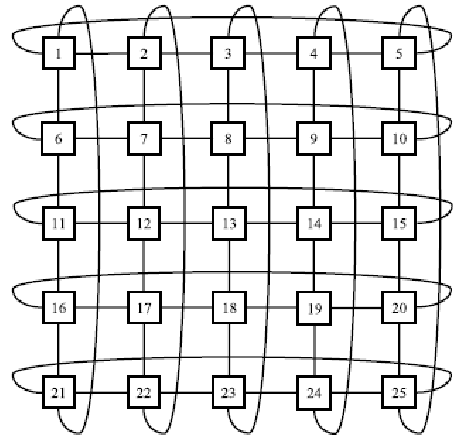
\includegraphics[width=.6\textwidth]{./images/torus-network-topology.png}
                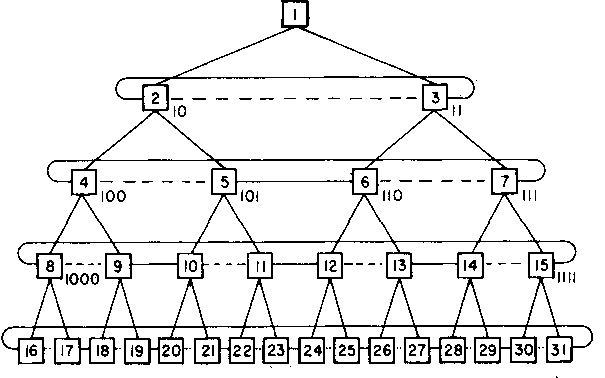
\includegraphics[width=.6\textwidth]{./images/binary-tree-network-topology.png}
                \caption{Two example target topologies: grid (top) and binary tree (bottom).}
            \end{figure}
        \end{column}
    \end{columns}

\end{frame}

\begin{frame}
    \frametitle{The \textsc{T-Man} Protocol}

    \vspace{-25pt}

    \SetKwRepeat{Do}{do}{while}
    \begin{figure}[h!]
    \centering
    \begin{minipage}[t]{.45\textwidth}
    \null 
     \begin{algorithm}[H]
        \DontPrintSemicolon
        \Do{true}{
            $p \gets$ selectPeer() \;
            send($p$, merge($view$, $rnd.view$)) \;
            $buffer \gets$ receive($p$) \;
            $view \gets $ merge($view$, $buffer$) \;
        }
        \caption{Active Thread}
      \end{algorithm}
    \end{minipage}%
    \begin{minipage}[t]{.45\textwidth}
    \null
     \begin{algorithm}[H]
        \DontPrintSemicolon
        \Do{true}{
            $buffer_q \gets$ receive($q$) \;
            $buffer \gets $ merge($view$, $rnd.view$) \;
            send($q$, $buffer$) \;
            $view \gets$ merge($buffer_q, view$) \;
        }
        \caption{Passive Thread}
      \end{algorithm}
    \end{minipage}
    \caption{The \textsc{T-Man} Protocol.}
    \end{figure}

    \vspace{-20pt}

    \begin{itemize}
        \item The \texttt{selectPeer} method uses a rank function to determin the best peer, and the \texttt{merge} one takes the $n$ top-ranked peers.
        \item Interesting to observe the use of a random view in the algorithm (more on that later).
    \end{itemize}

\end{frame}

\begin{frame}
    \frametitle{Experiments}
    \framesubtitle{Or should I say simulations?}

    \textbf{Simulation Experiments:}
    \begin{itemize}
        \item Simulations done using \textit{PeerSim} on large networks.
        \item Authors compare three distance-based rank functions: linear, binary tree, and torus.
        \item They measure convergence and missing links to achieve target topology.
    \end{itemize}

    \begin{figure}[h!]
        \centering
        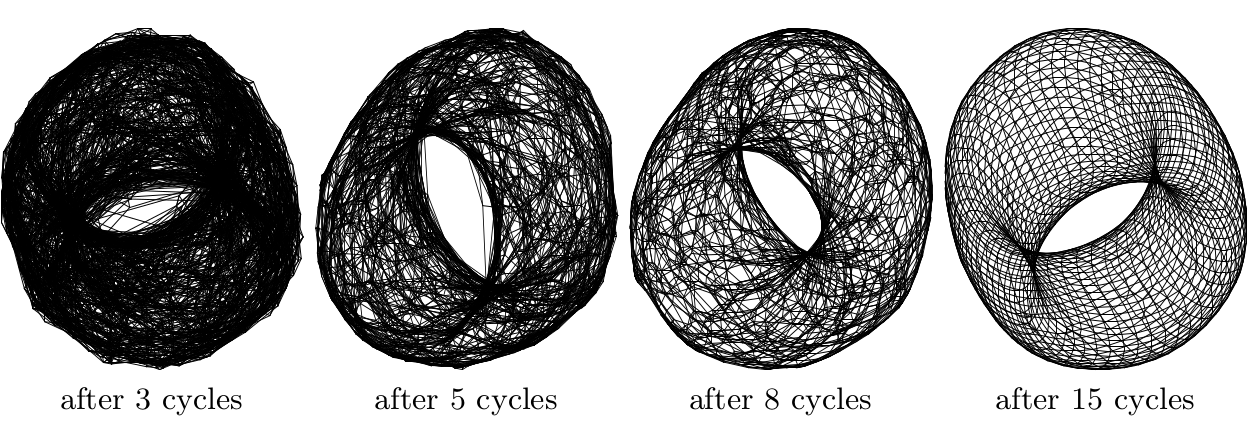
\includegraphics[width=.6\textwidth]{./images/convergence.png}
        \caption{Figure about the convergence to a torus (3D grid) w/ 2500 nodes.}
    \end{figure}
\end{frame}

\begin{frame}
    \frametitle{Experiments}
    \framesubtitle{Results}

    \textbf{Simulation Results:}
    \begin{itemize}
        \item Authors report logarithmic convergence with respect to network size.
        \item Full topology convergence is slower as some links are \textit{"hard"} to get.
    \end{itemize}

    \begin{figure}[h!]
        \centering
        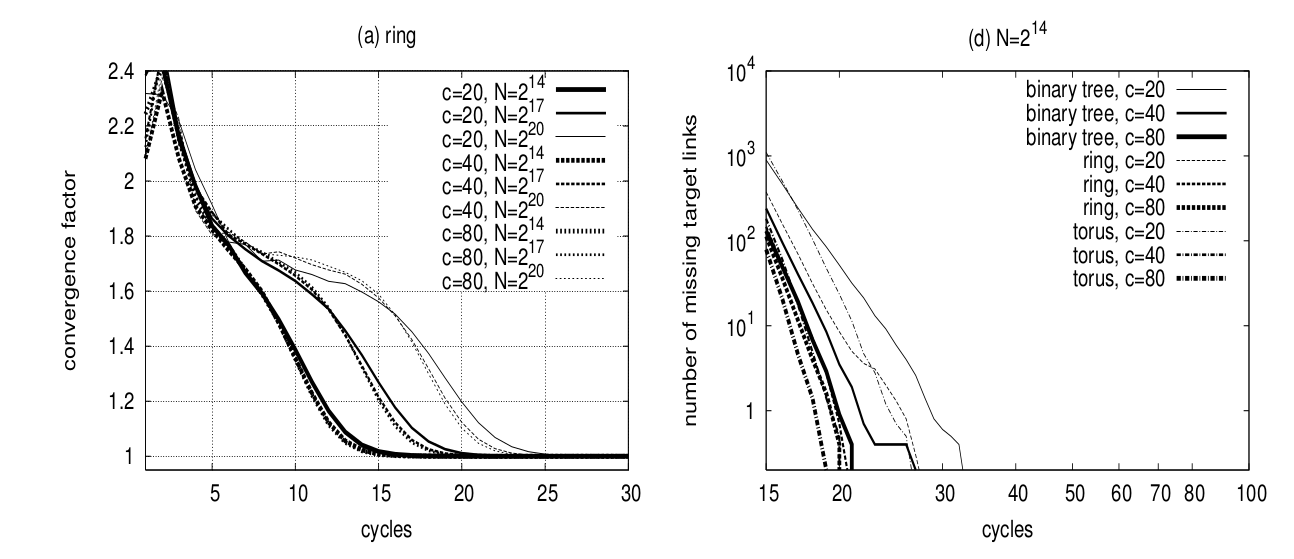
\includegraphics[width=.6\textwidth]{./images/ring-results.png}
        \caption{Results for the experiment in the ring topology.}
    \end{figure}
\end{frame}

\begin{frame}
    \frametitle{Network Churn}
    \framesubtitle{Definition, Importance, and Solution}

    One of the biggest motivations for the work was to be able to deal with \textbf{network churn}.
    \begin{itemize}
        \item \textbf{\textcolor{blue}{Netowrk churn}} happens when nodes constantly leave and join the network.
        \item How can we achieve our target topology (or maintain it) in such scenario?
        \begin{itemize}
            \item Authors introduce an \textit{aging} factor in the rank function, to discard \textbf{dead} links.
            \item Convergence is still reasonable even under high churn rates.
        \end{itemize}
    \end{itemize}
    The authors say that they are working in using \textsc{T-Man} in existing DHT implementations to provide with \textbf{robustness} in the event of massive failures and extreme churn.
    \begin{itemize}
        \item Is churn something current decentralized protocols are still worried about?
    \end{itemize}
\end{frame}

\begin{frame}
    \frametitle{Open Questions}

    Lastly, \textbf{some questions:}
    \begin{enumerate}
        \item Do you think gossip protocols still play a role in nowadays decentralized systems?
        \item Why do you think the authors include a random view in the algorithm? What is it used for?
        \item Very often, the mathematics of epidemics are used to model gossip communications. Do you think our experience with gossip protocols could help us better understand the current pandemic? (Open question: do you think there exists a feedback relation between models that mimic natural behaviours, once these are put in production and stressed?)
    \end{enumerate}

\end{frame}



\end{document}
